\documentclass{siproblemset}

\usepackage{multicol}
\usepackage{xcolor}
\usepackage{mathtools}
\usepackage{graphicx}
\usepackage{siunitx}

% SI Session Information
\course{MTH 1321}
\sessionnum{PT2}
\sessiondate{10/13/21}

% Worksheet Information
\title{Practice Test \#2}
\sections{Chapter 3}
\withnamespace

\definecolor{darkred}{RGB}{110,0,0}

%\debugmode

\begin{document}
    \maketitle
    
    \begin{center}
    \framebox{
        \begin{minipage}{\textwidth}
            \begin{center}
                \textbf{When completing this practice test, do your best to mimic the test environment:}
            \end{center}
            \begin{enumerate}
                \item Do not use a calculator.
                \item Try not to use your notes.
                \item Time yourself, make sure you are completing the problems at a comfortable pace. Remember that you will only get \textbf{2 hours} for the actual exam (with fewer questions of course).
                \item The answer key will be available at the test review session on \textbf{3/8/22 from 5:30-7:30 pm}.
                \item If you have any questions, feel free to email me at {\color{blue} Matthew\_McCaskill1@baylor.edu}.
            \end{enumerate}
        \end{minipage}
    }
    \end{center}

    \newpage

    \begin{multipartquestion}{Use the graph of $f(x)$ below to answer the following questions.}
        \begin{multicols}{2}
            \begin{center}
                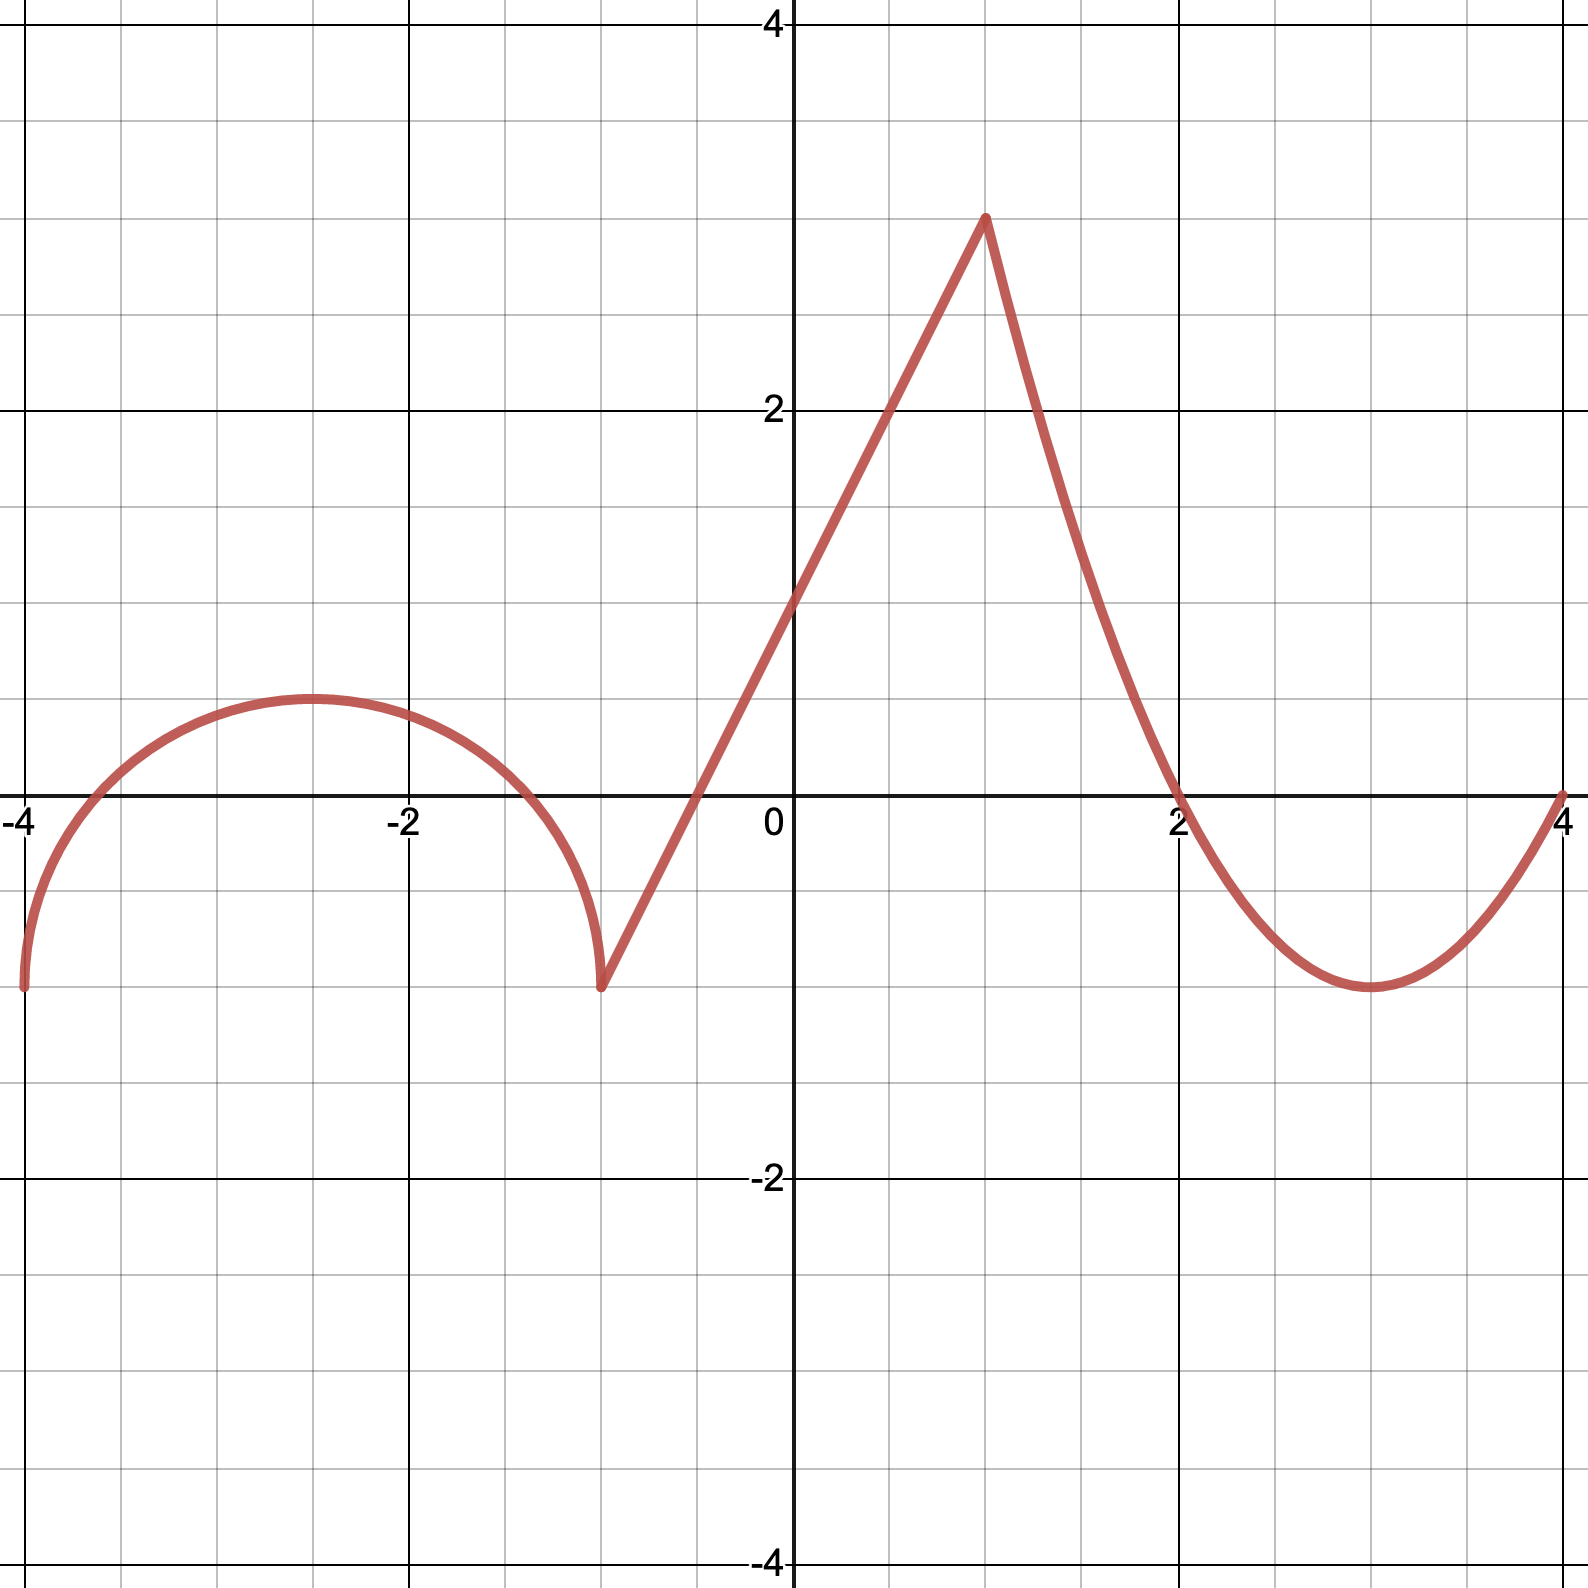
\includegraphics[width=\linewidth]{img/pt2-graph1}
            \end{center}
            \frq{On which interval(s) is $f'(x)$ positive?}
            \tinysp
            \frq{On which interval(s) is $f'(x)$ negative?}
            \tinysp
            \frq{What is $f'(0)$?}
            \tinysp
            \frq{At which $x$-value(s) does $f(x)$ have a horizontal tangent line?}
            \tinysp
        \end{multicols}
        \begin{multicols}{2}
            \frq{At which $x$-value(s) does $f'(x)$ not exist?}
            \tinysp
        \end{multicols}
    \end{multipartquestion}
    \tinysp

    \begin{multipartquestion}{Use the graph of $f'(x)$ below to answer the following questions.}
        \begin{multicols}{2}
            \begin{center}
                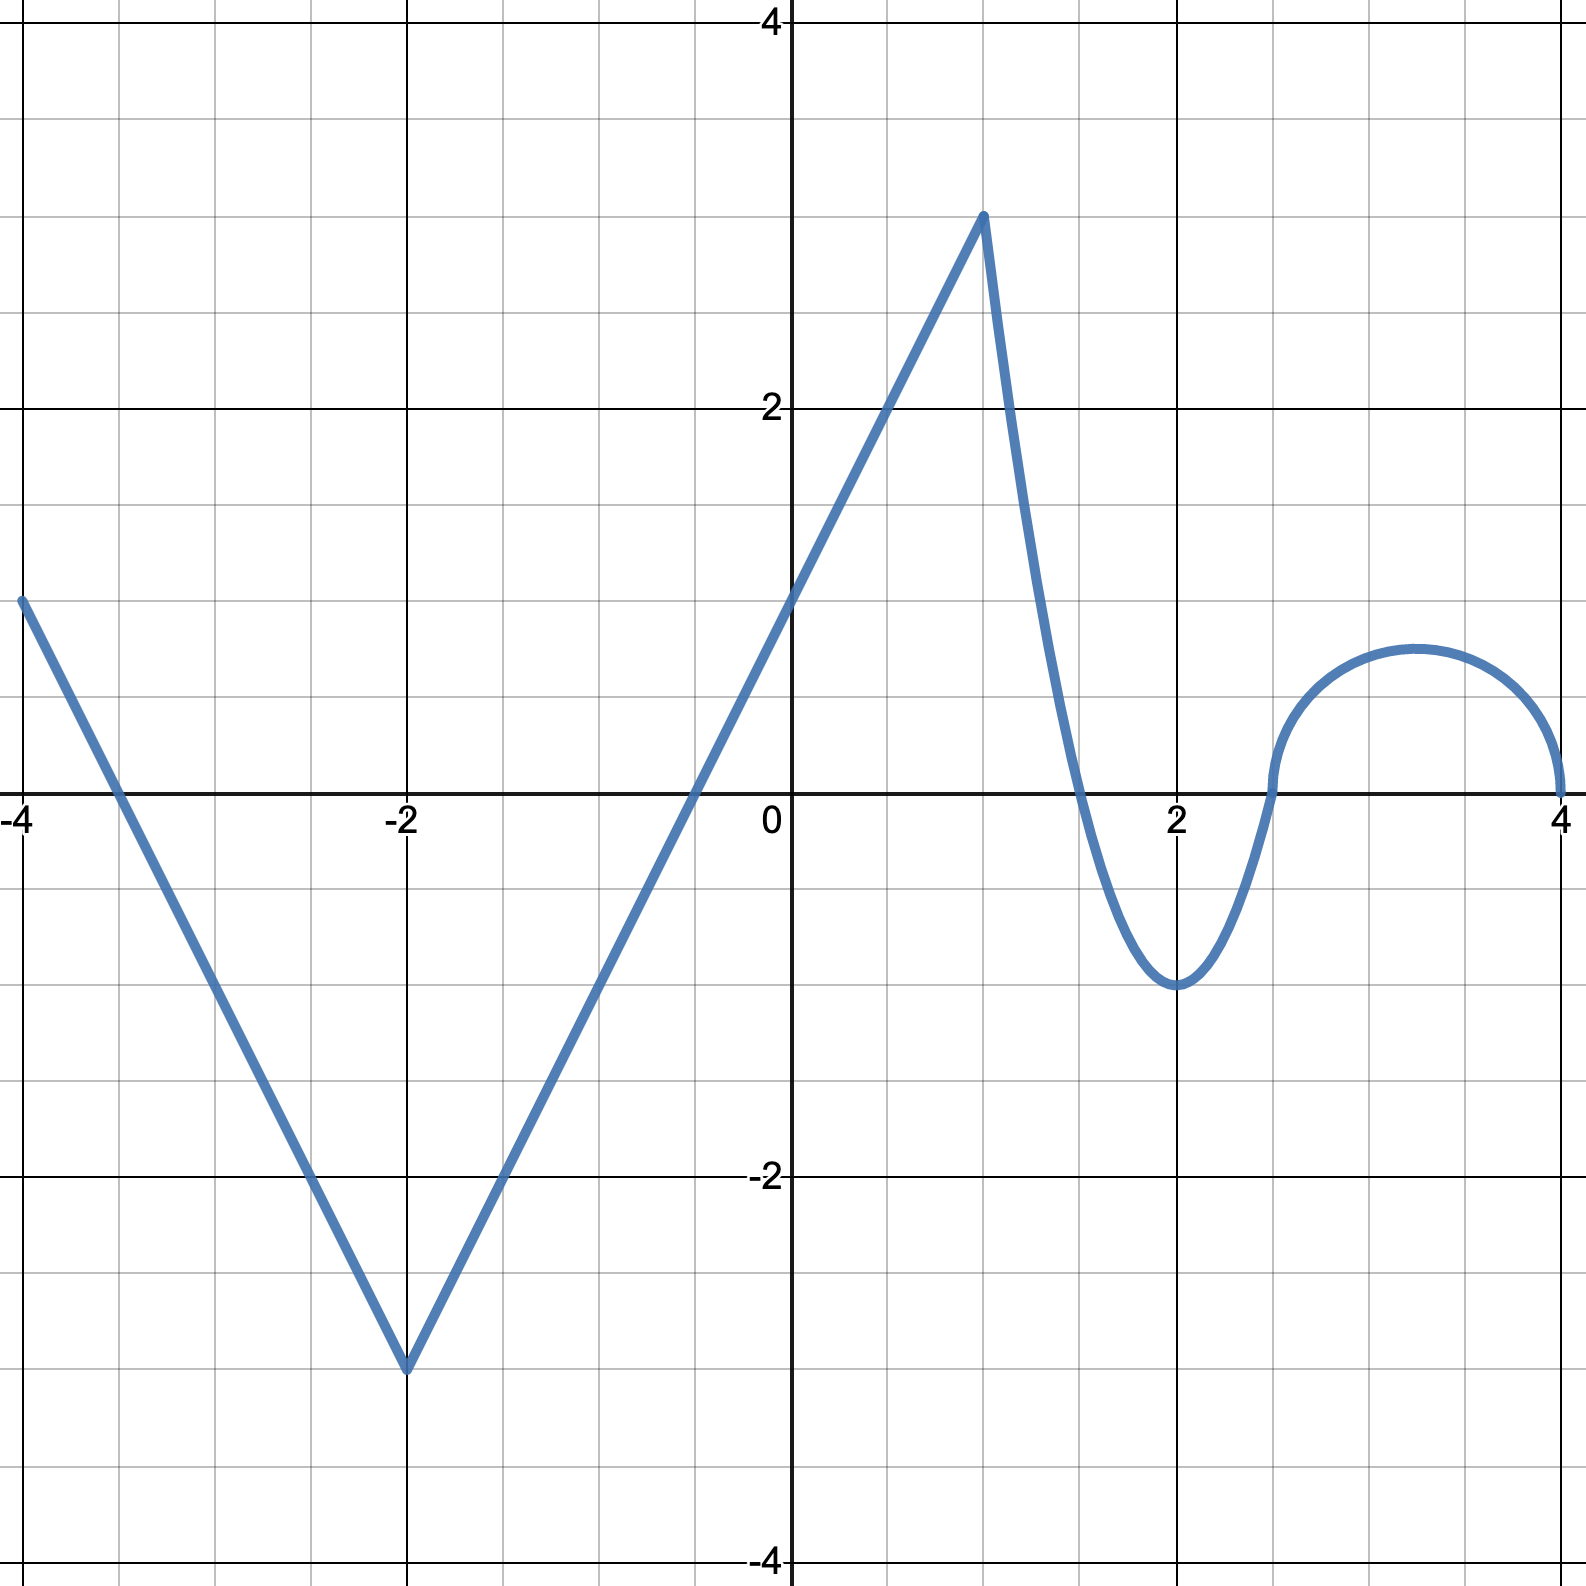
\includegraphics[width=\linewidth]{img/pt2-graph2}
            \end{center}
            \frq{On which interval(s) is $f(x)$ increasing?}
            \tinysp
            \frq{On which interval(s) is $f(x)$ decreasing?}
            \tinysp
            \frq{At which $x$-value(s) does $f(x)$ have a horizontal tangent line?}
            \tinysp
        \end{multicols}
    \end{multipartquestion}
    \newpage
    
    \mcq{I am a master archer. To prove this, I want to throw an apple straight into the air and shoot it with an arrow. I throw the apple into the air and shoot my arrow. I estimate that the arrow hit the apple when the apple was about 10 meters off the ground after about 1 second.}{
        \task What was the initial velocity of the arrow?
        \Smallsp
        \task What was the velocity of the arrow at the moment that it hit the apple?
        \Smallsp
        \task Assuming that the arrow passed straight through the apple without losing any speed or changing course, what would the maximum height of the arrow be?
        \Smallsp
        \task How long would it take for the arrow to hit the ground (i.e. total time in the air from firing the arrow to it hitting the ground)?
    }
    \newpage

    \mcq{A 17ft ladder is leaning against a building. The foot of the ladder is 8ft from the base of the building and it's sliding away from the building at 3ft/s.}{
        \task How fast is the top of the ladder sliding down the wall of the building?
        \Hugesp
        \task How fast is the area formed by the ladder changing at this instant?
    }
    \newpage
    
    \mcq{Compute $f'(x)$ \textbf{using the limit definition of the derivative}. \underline{Simplify your final answer}.}{
        \task $f(x)=\sqrt{3x-2}$
        \Hugesp
        \task $f(x)=-\dfrac{3}{(x-3)^2}$
    }
    \newpage
    
    \begin{multipartquestion}{Below are the graphs of three functions, $f(x)$, $g(x)$, and $h(x)$, their derivatives, $f'(x)$, $g'(x)$, and $h'(x)$, and their second derivatives, $f''(x)$, $g''(x)$, $h''(x)$. Determine which of each of the below graphs correspond to the listed functions below. You may choose which triplet you call "$f(x)$", which one you call "$g(x)$", and which one you call "$h(x)$". }
        \begin{multicols}{3}
            \begin{center}
                Graph A
                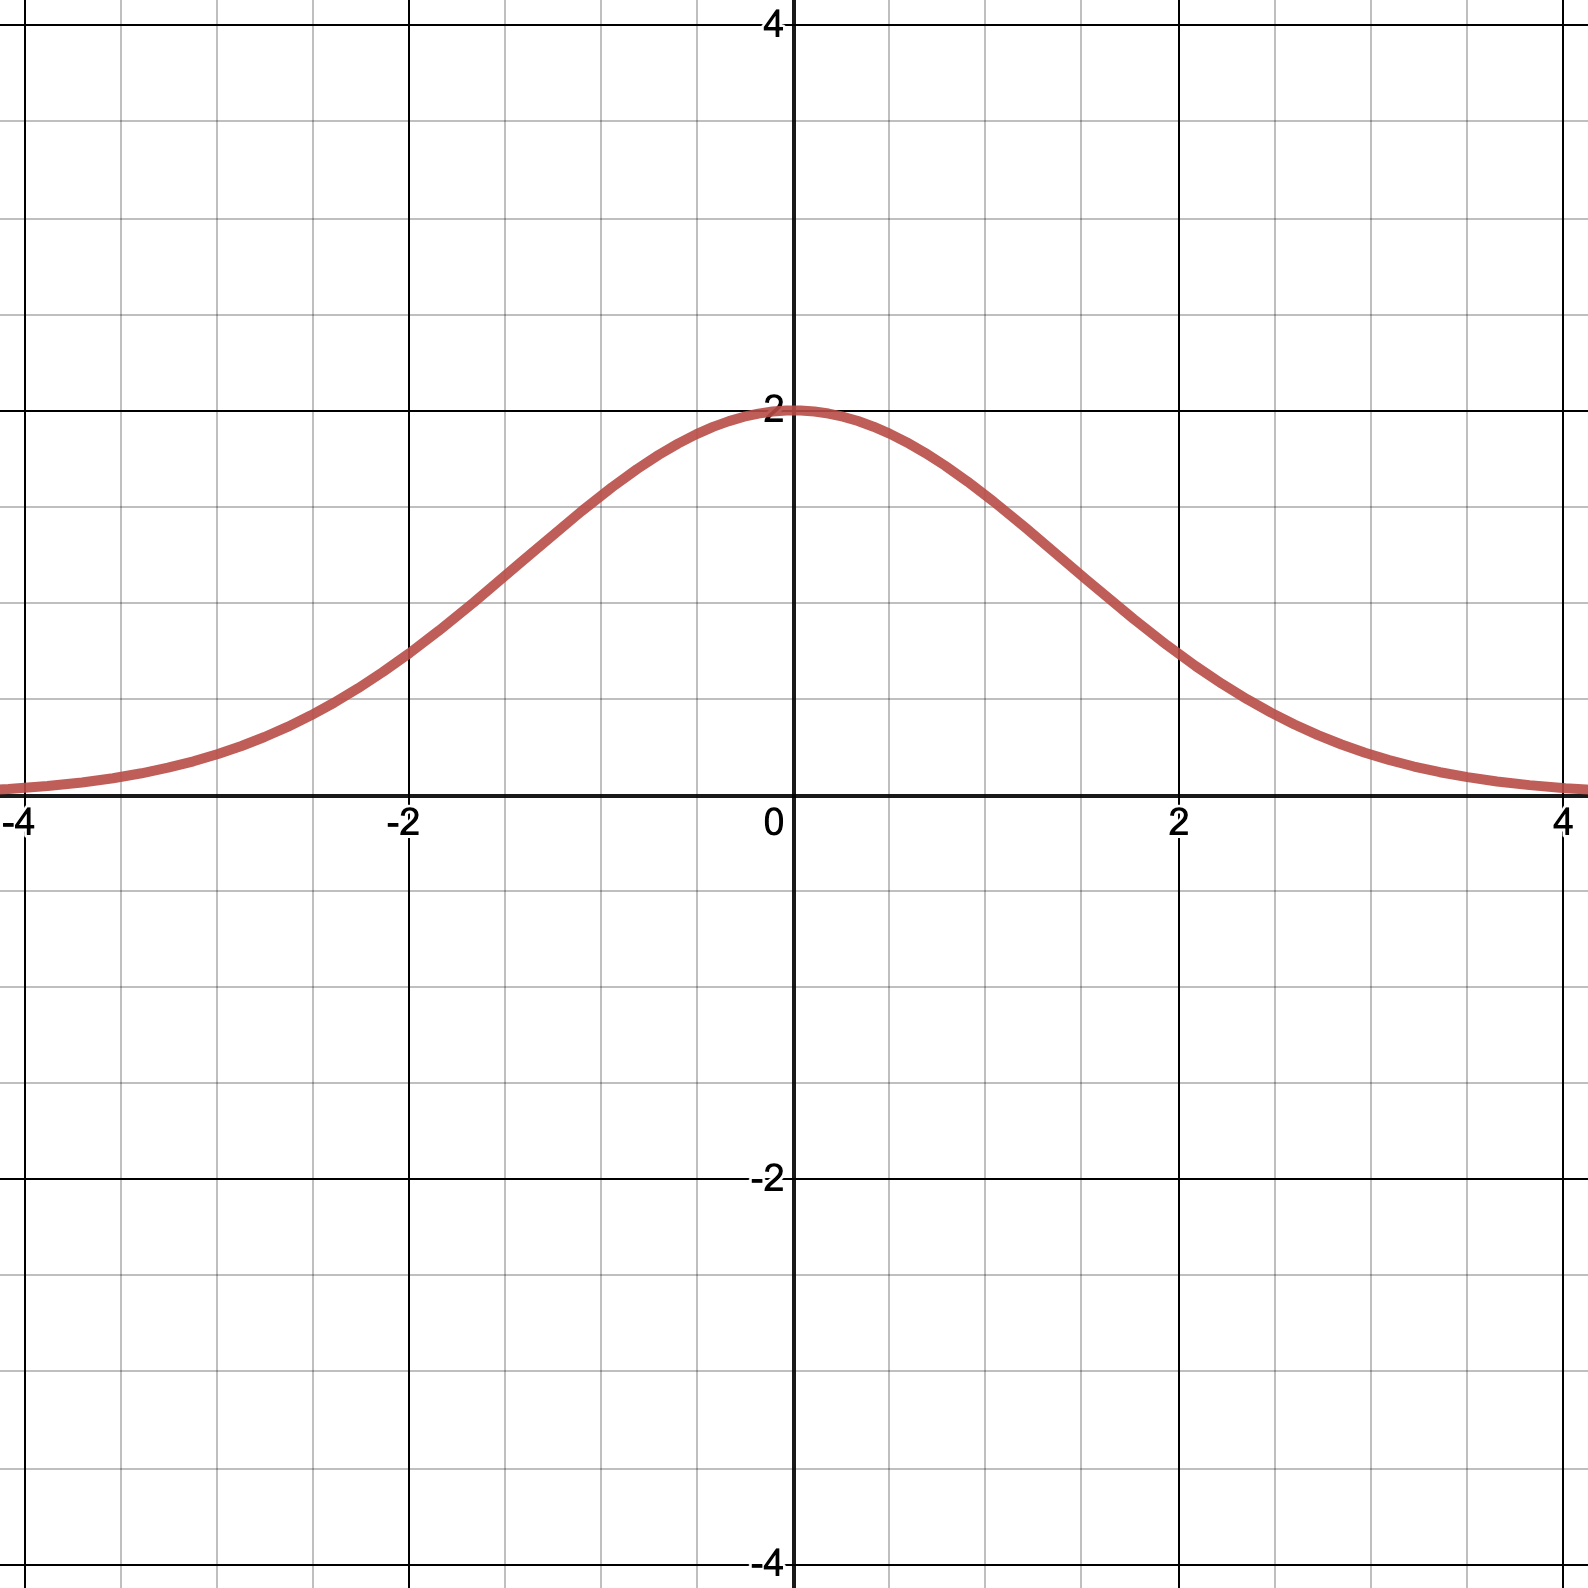
\includegraphics[width=\linewidth]{img/pt2-graph3a}
            \end{center}
            \begin{center}
                Graph D
                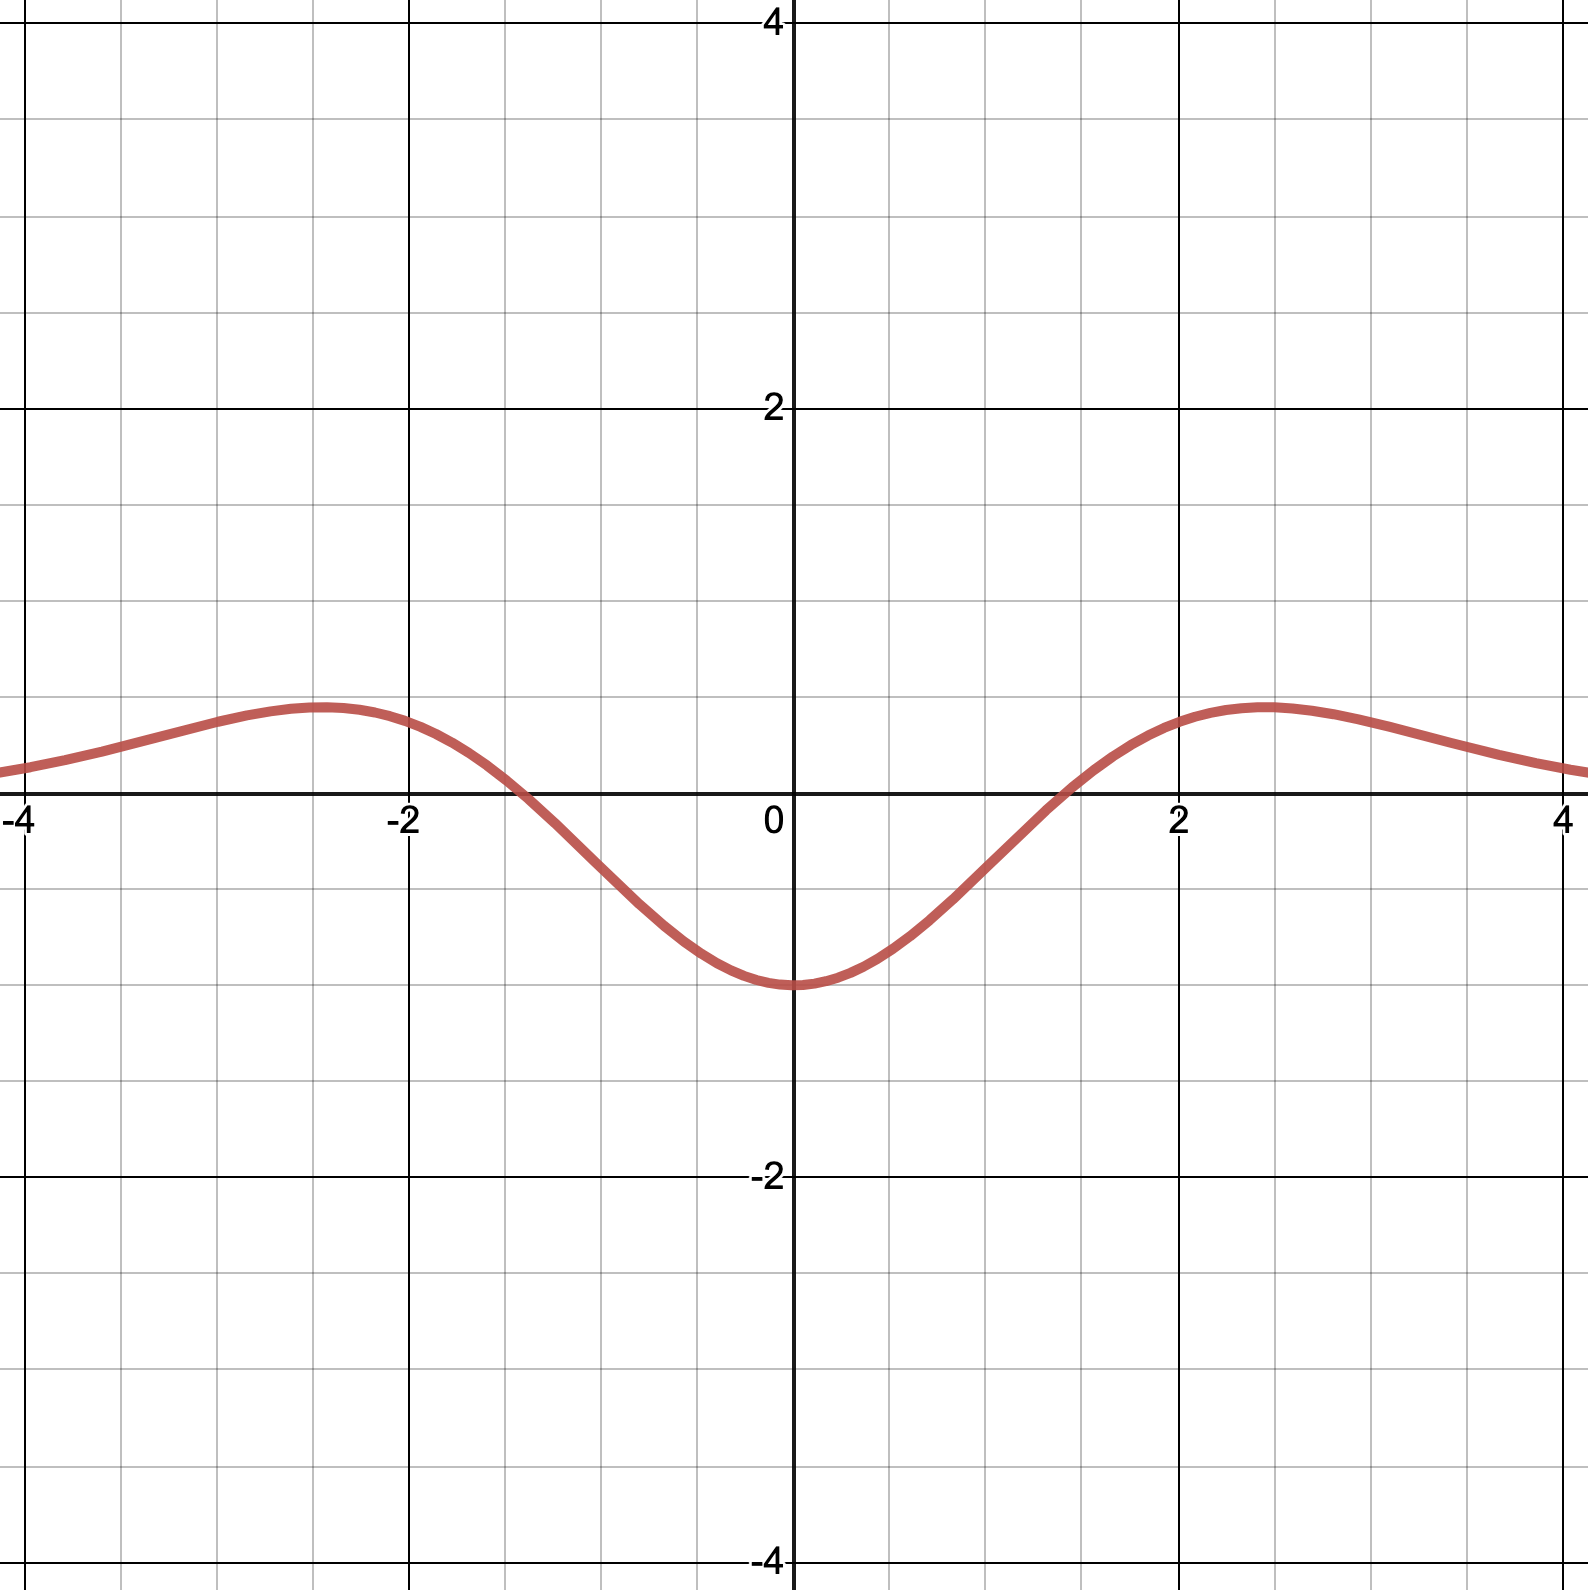
\includegraphics[width=\linewidth]{img/pt2-graph3c}
            \end{center}
            \begin{center}
                Graph G
                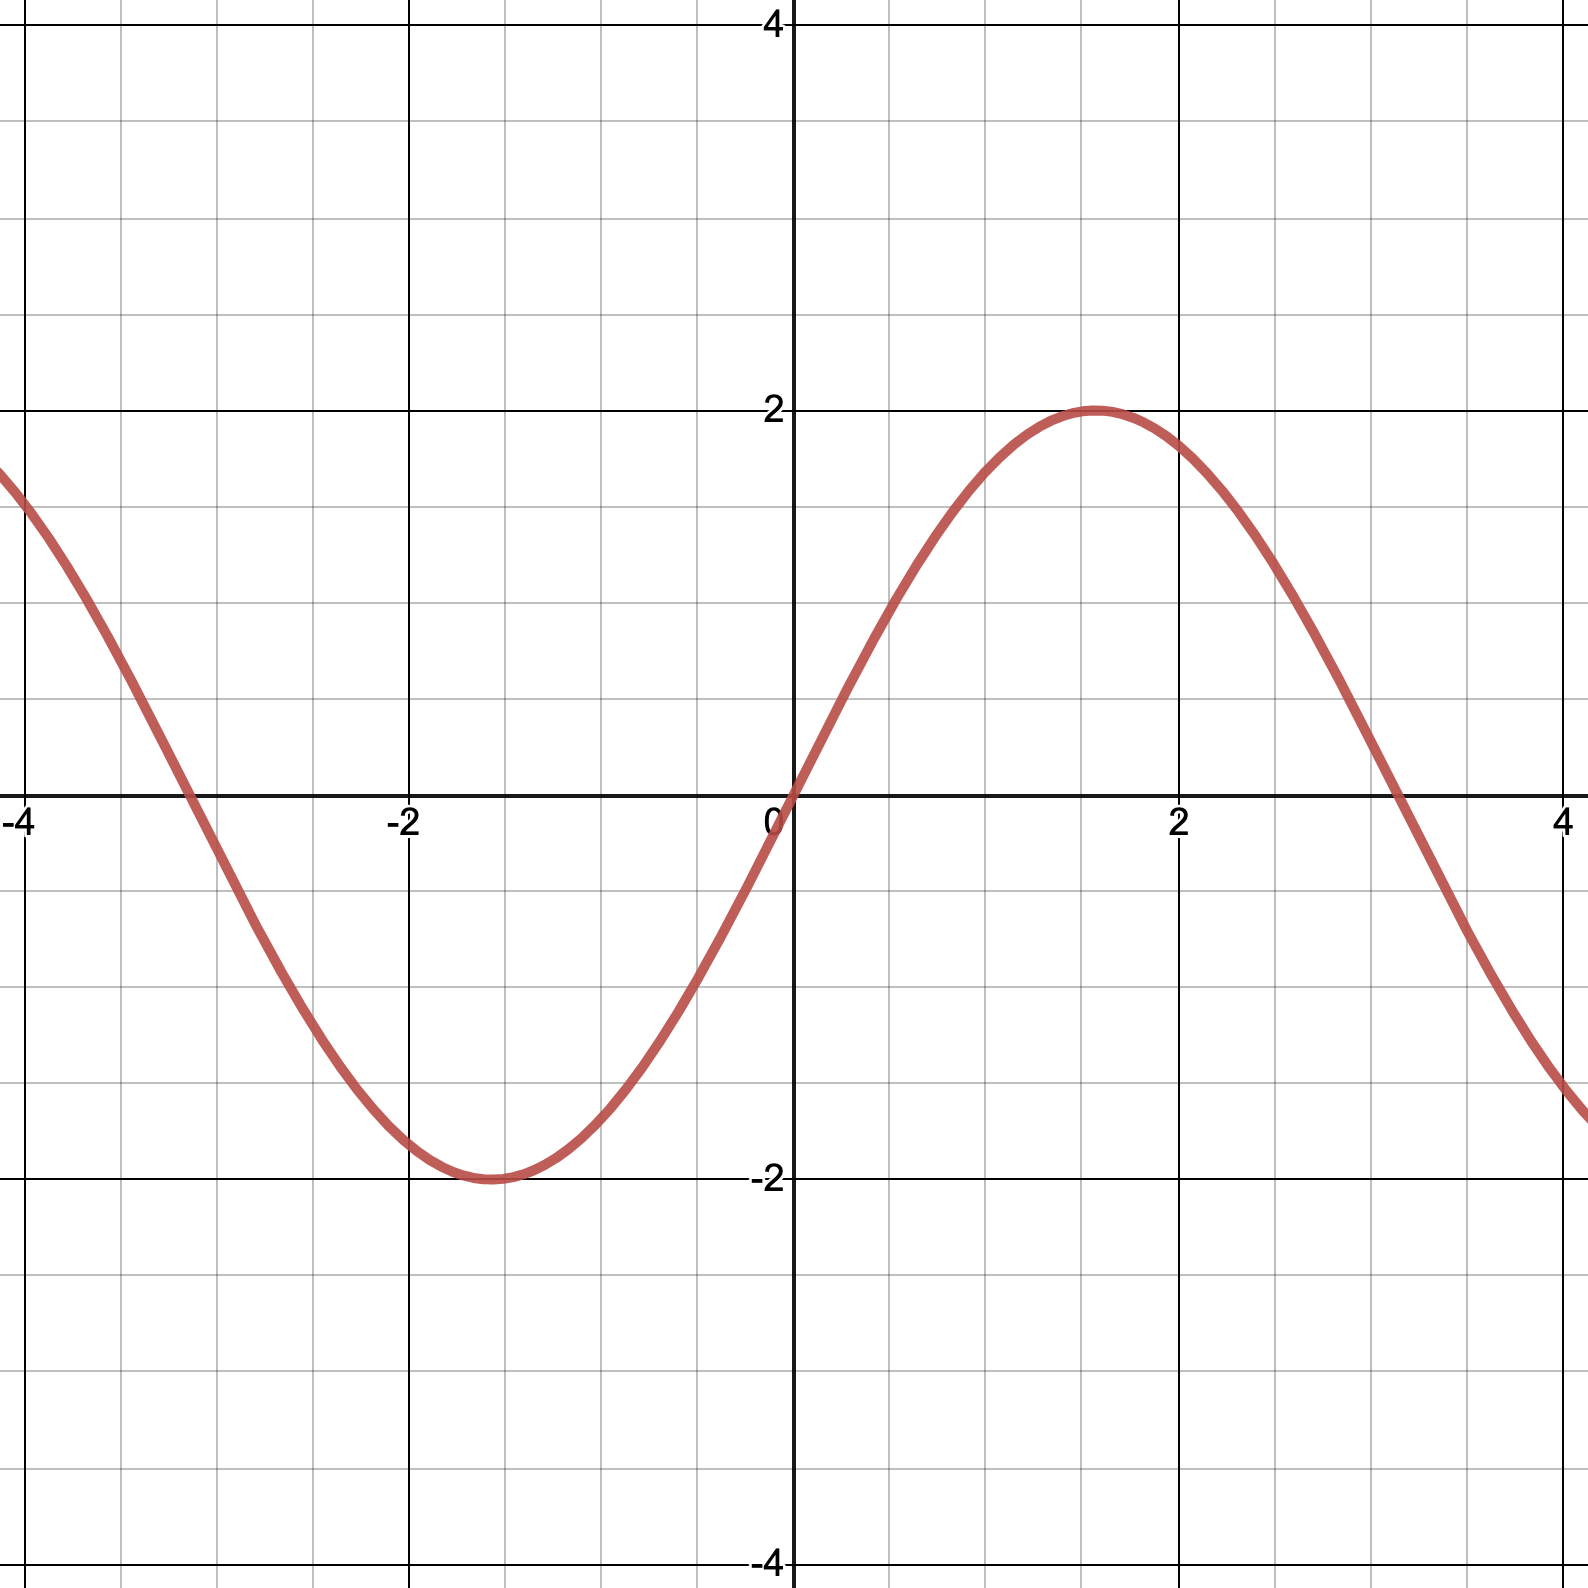
\includegraphics[width=\linewidth]{img/pt2-graph3g}
            \end{center}
            \begin{center}
                Graph B
                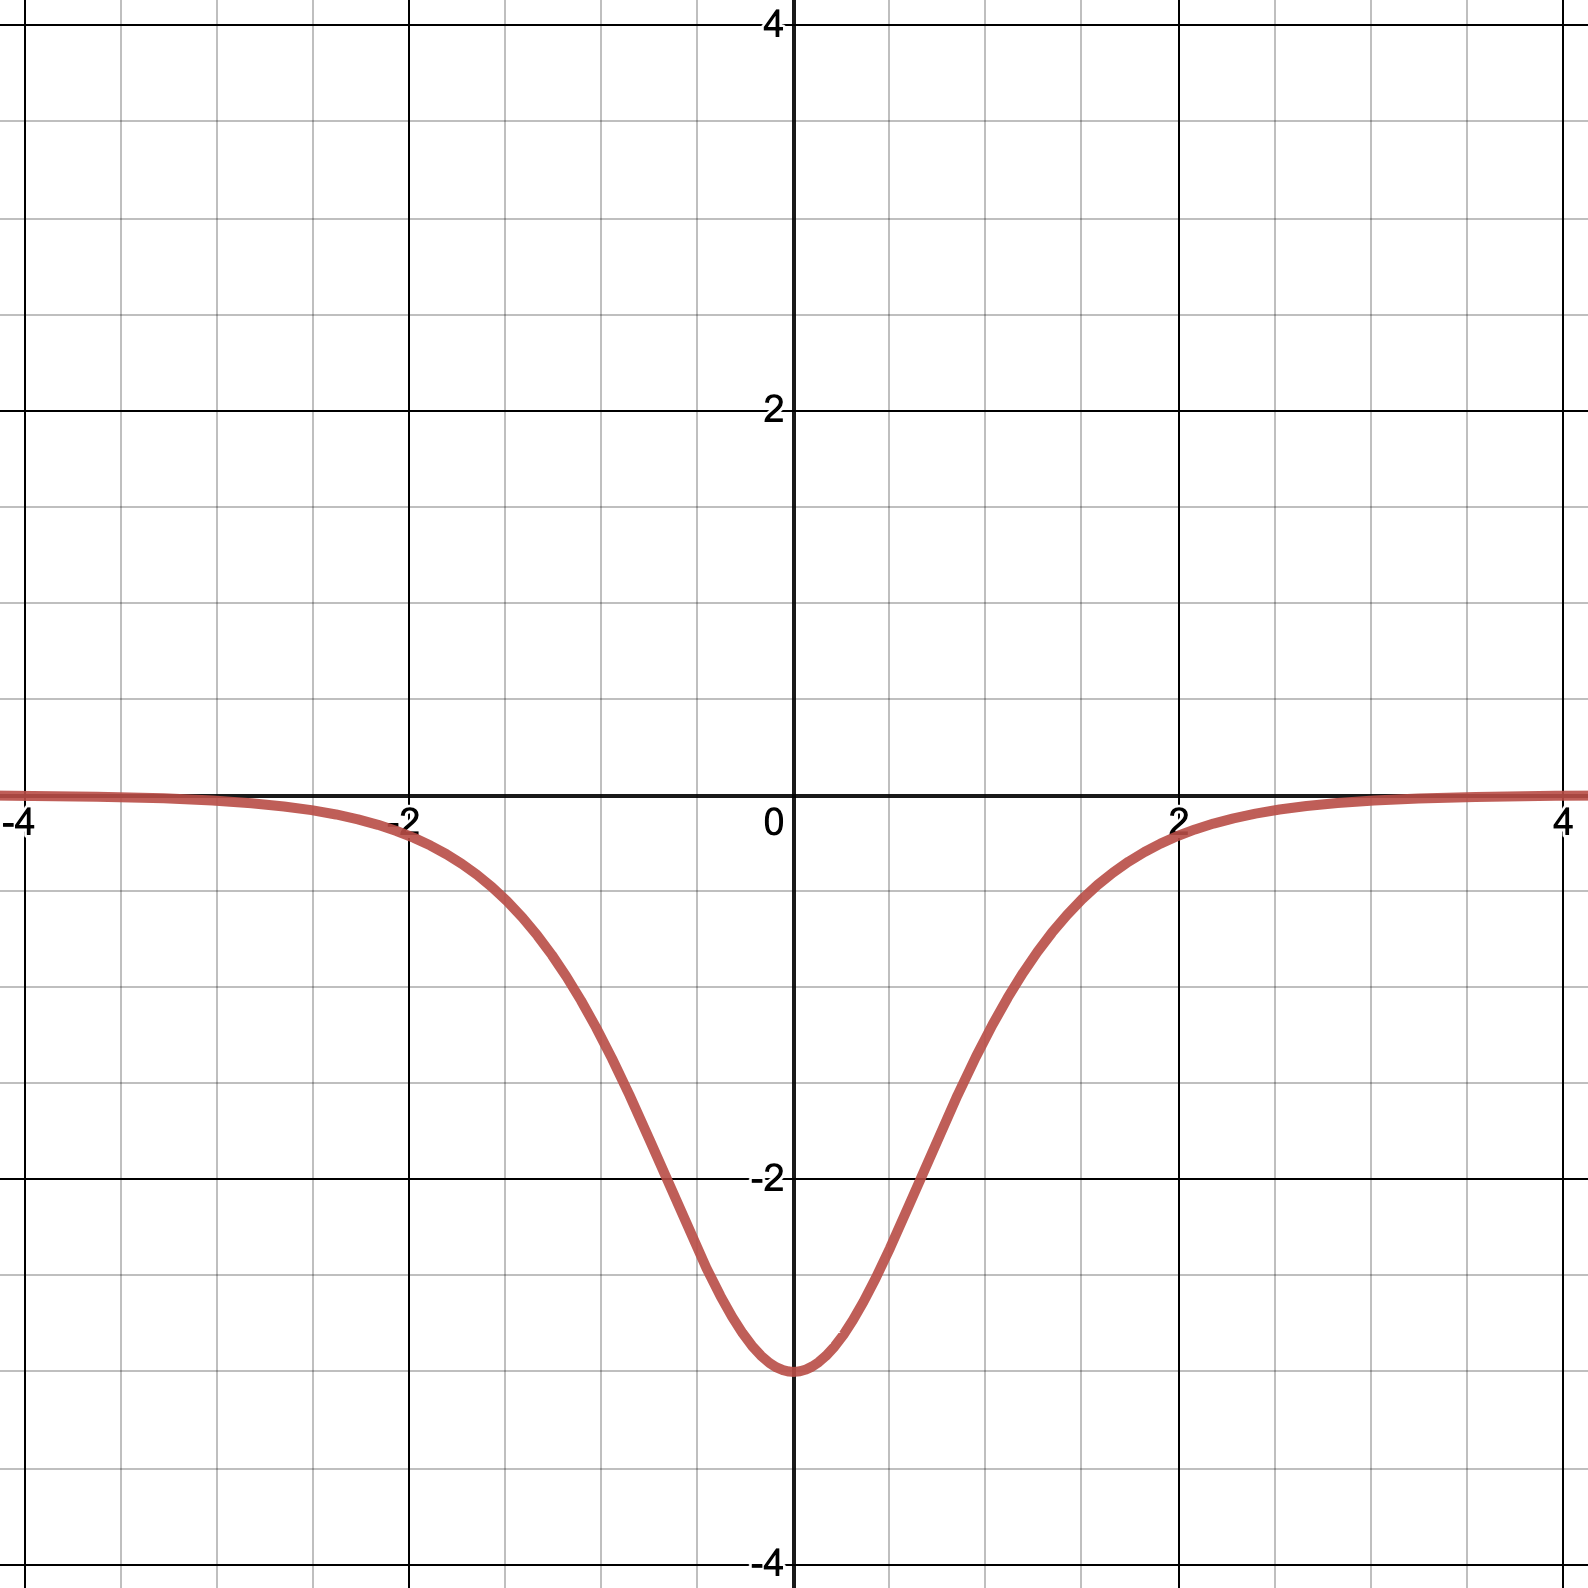
\includegraphics[width=\linewidth]{img/pt2-graph3e}
            \end{center}
            \begin{center}
                Graph E
                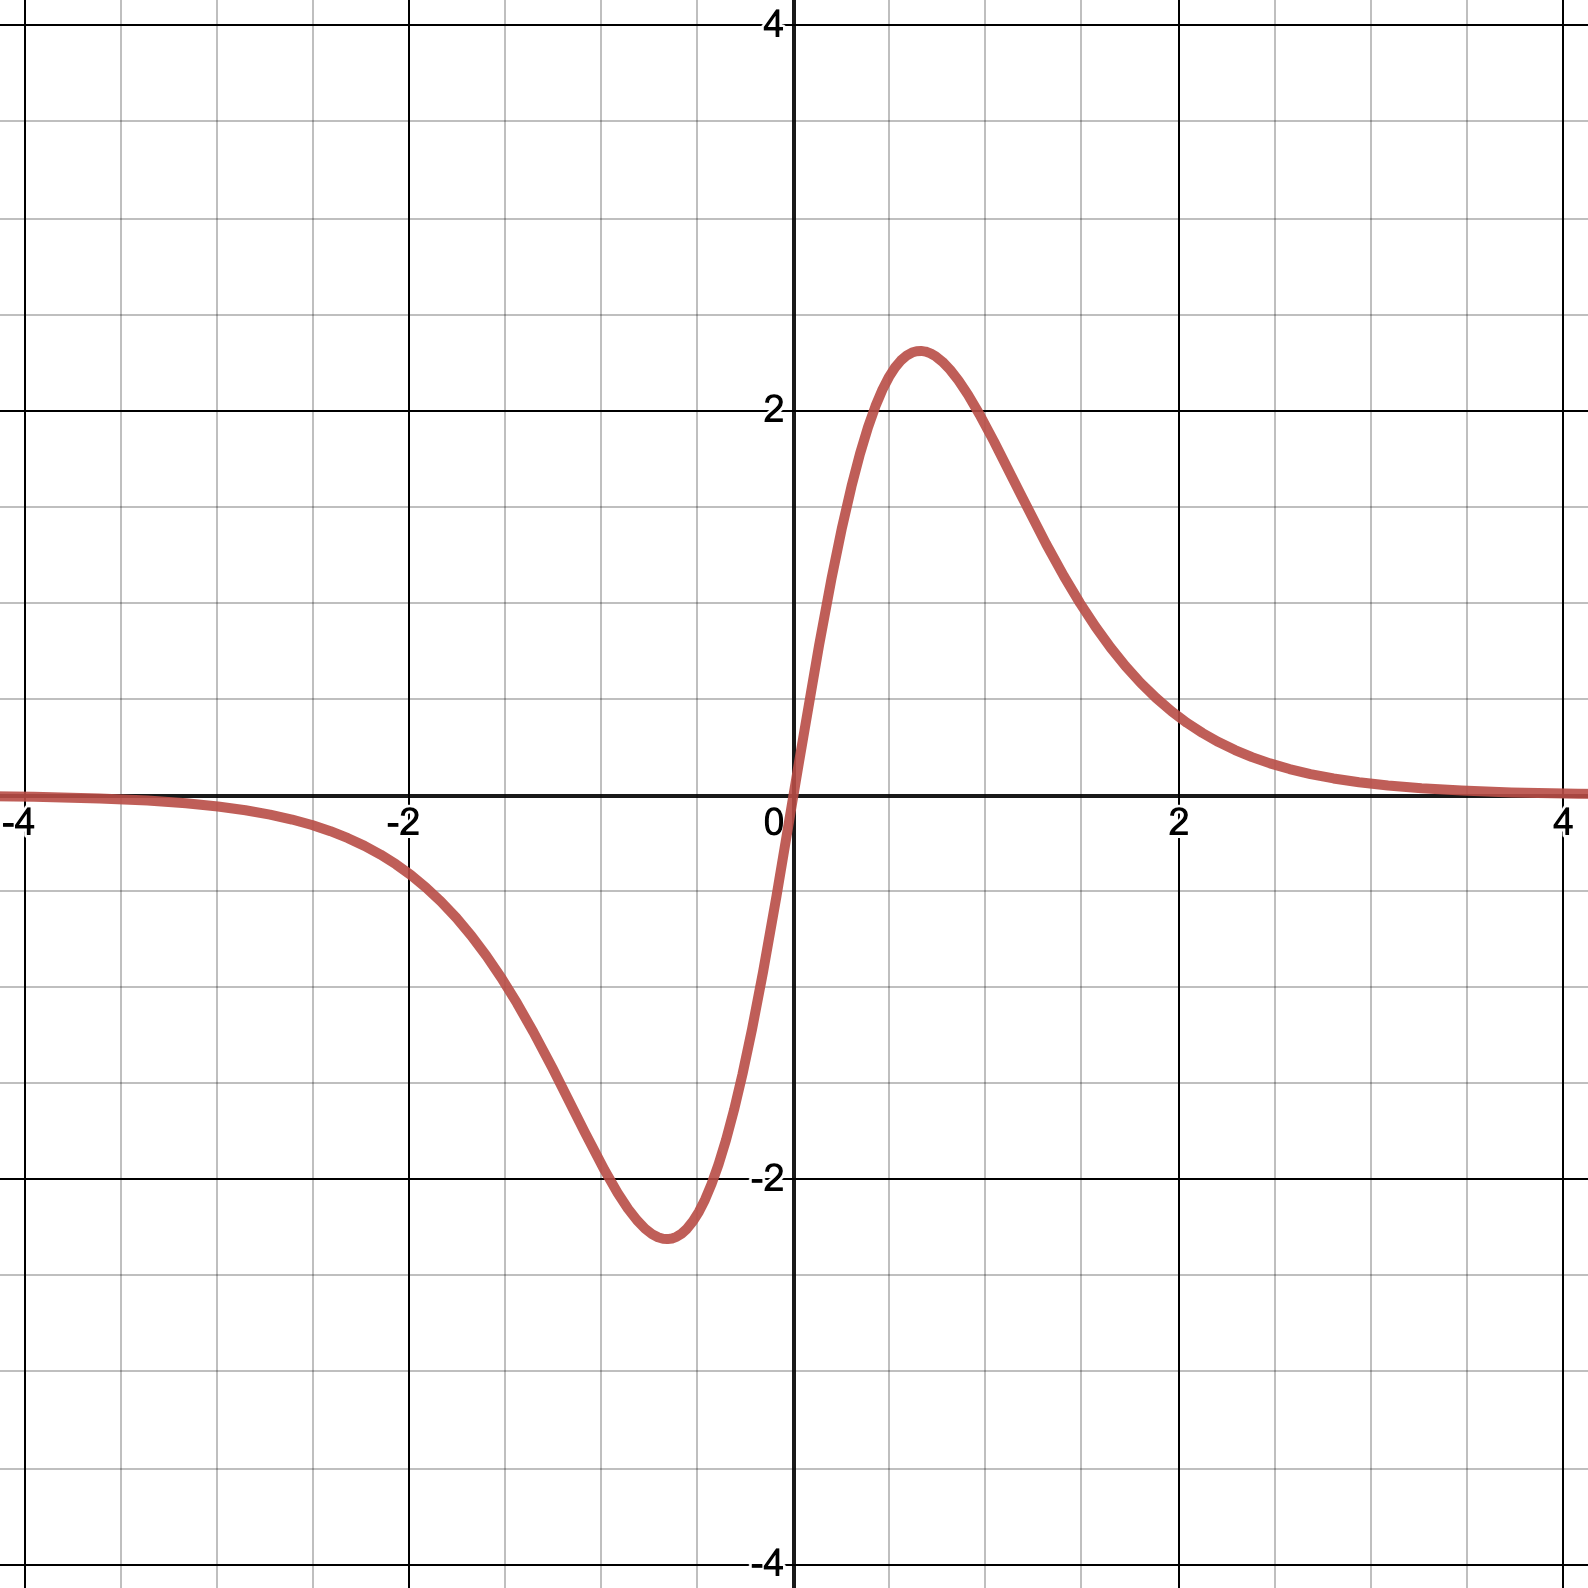
\includegraphics[width=\linewidth]{img/pt2-graph3f}
            \end{center}
            \begin{center}
                Graph H
                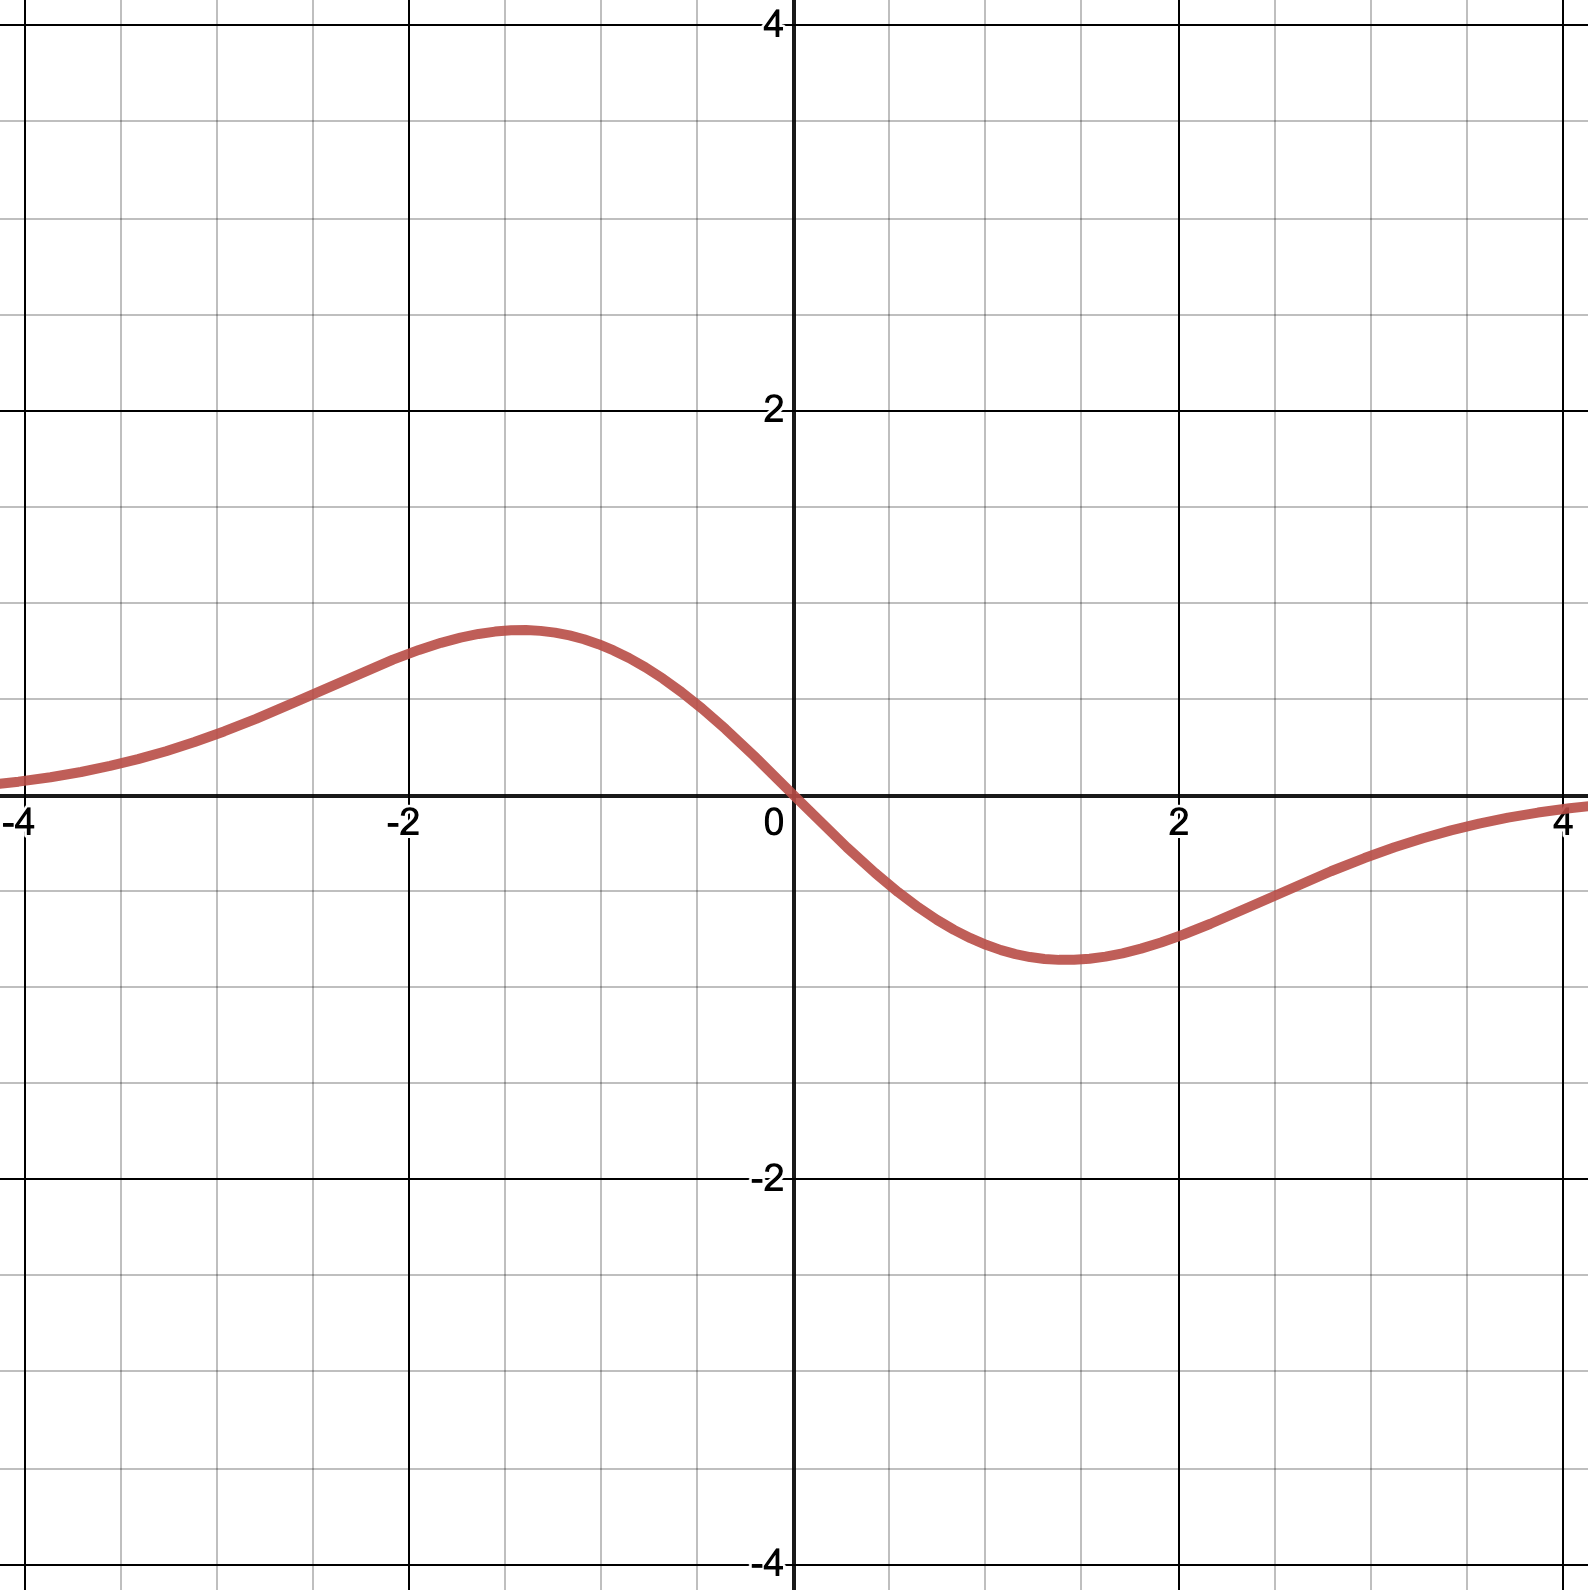
\includegraphics[width=\linewidth]{img/pt2-graph3b}
            \end{center}
            \begin{center}
                Graph C
                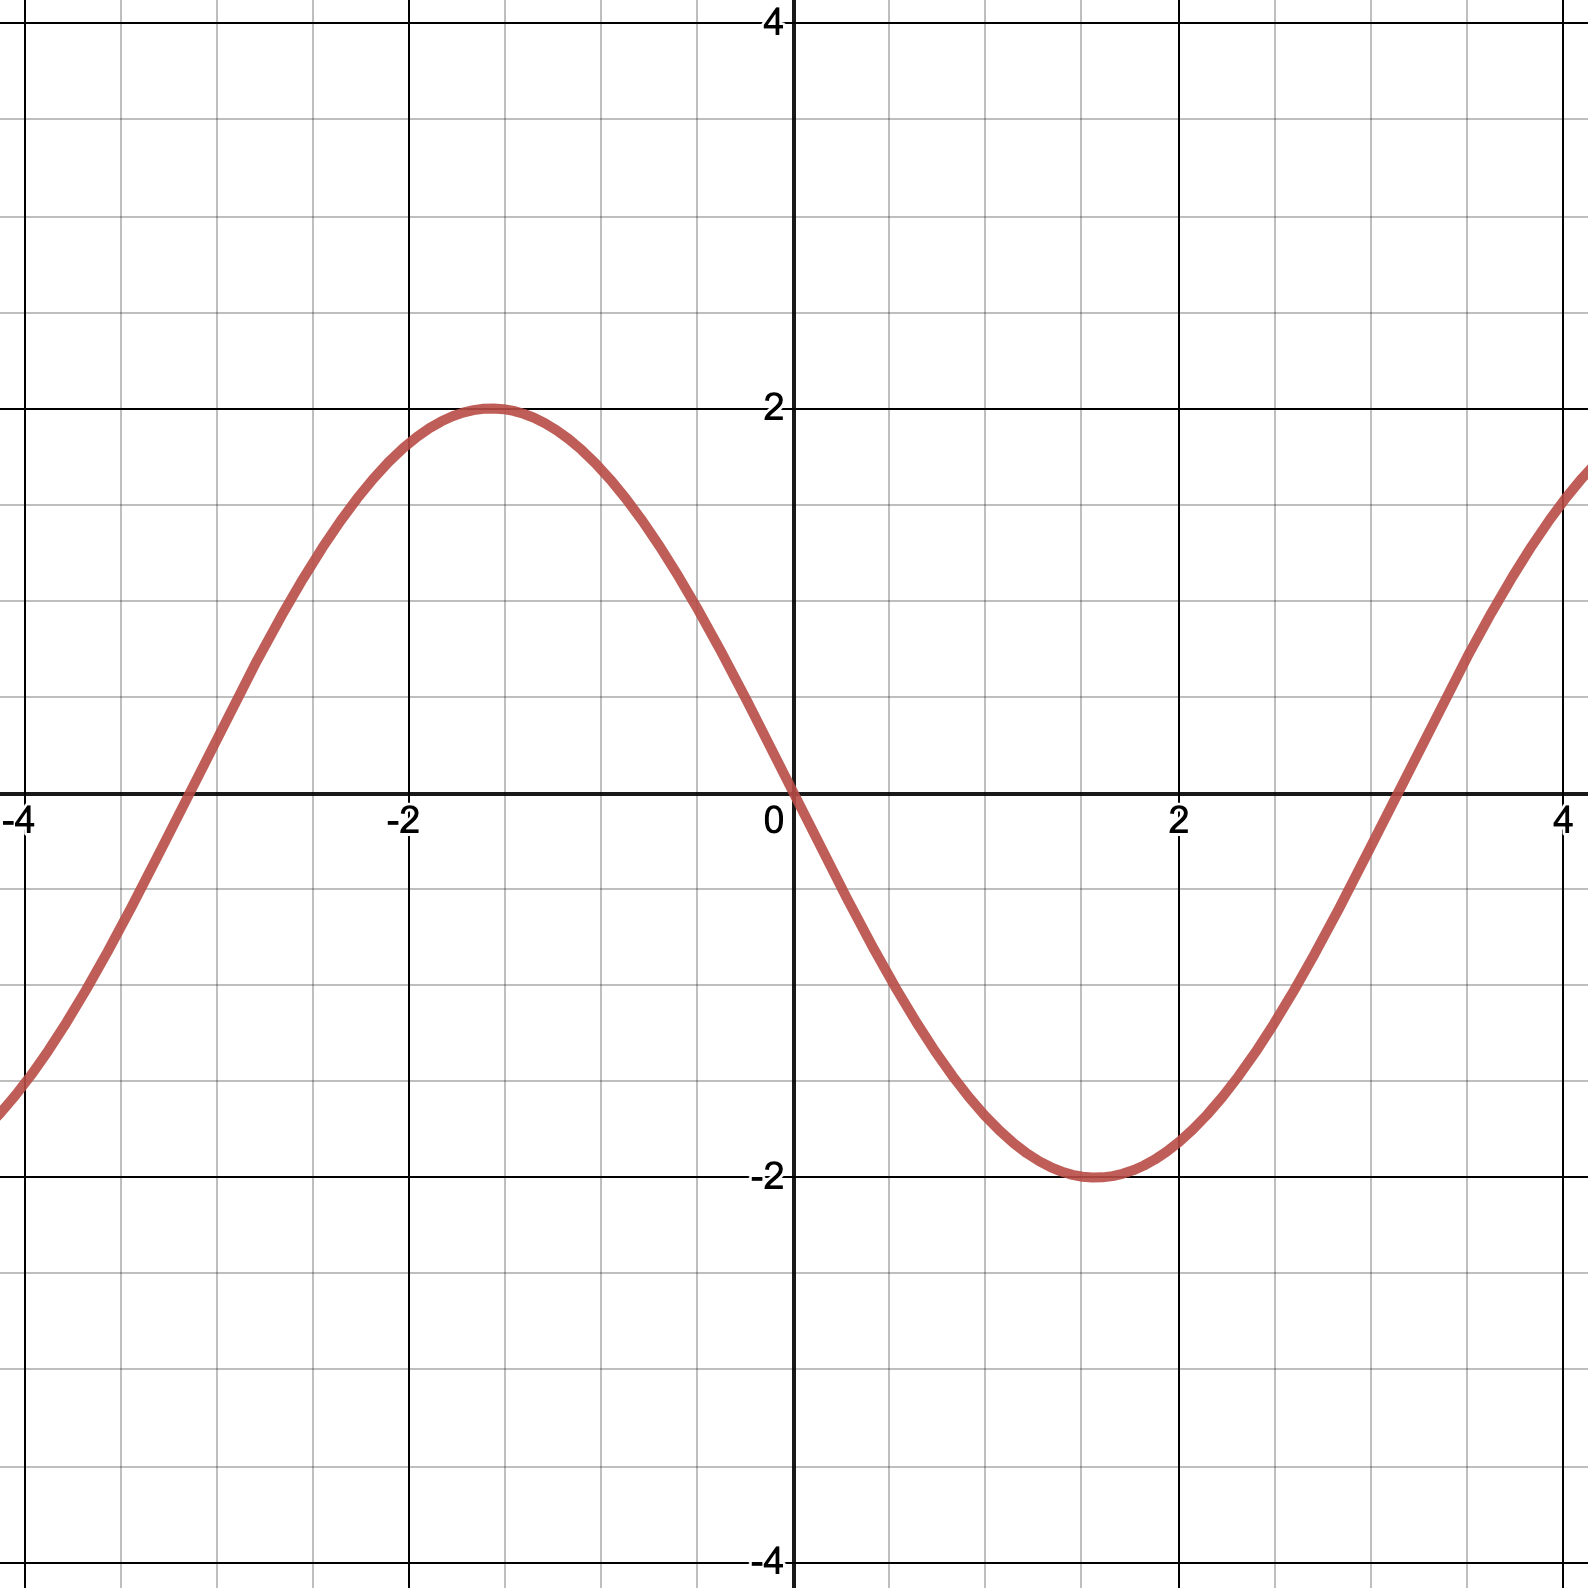
\includegraphics[width=\linewidth]{img/pt2-graph3i}
            \end{center}
            \begin{center}
                Graph F
                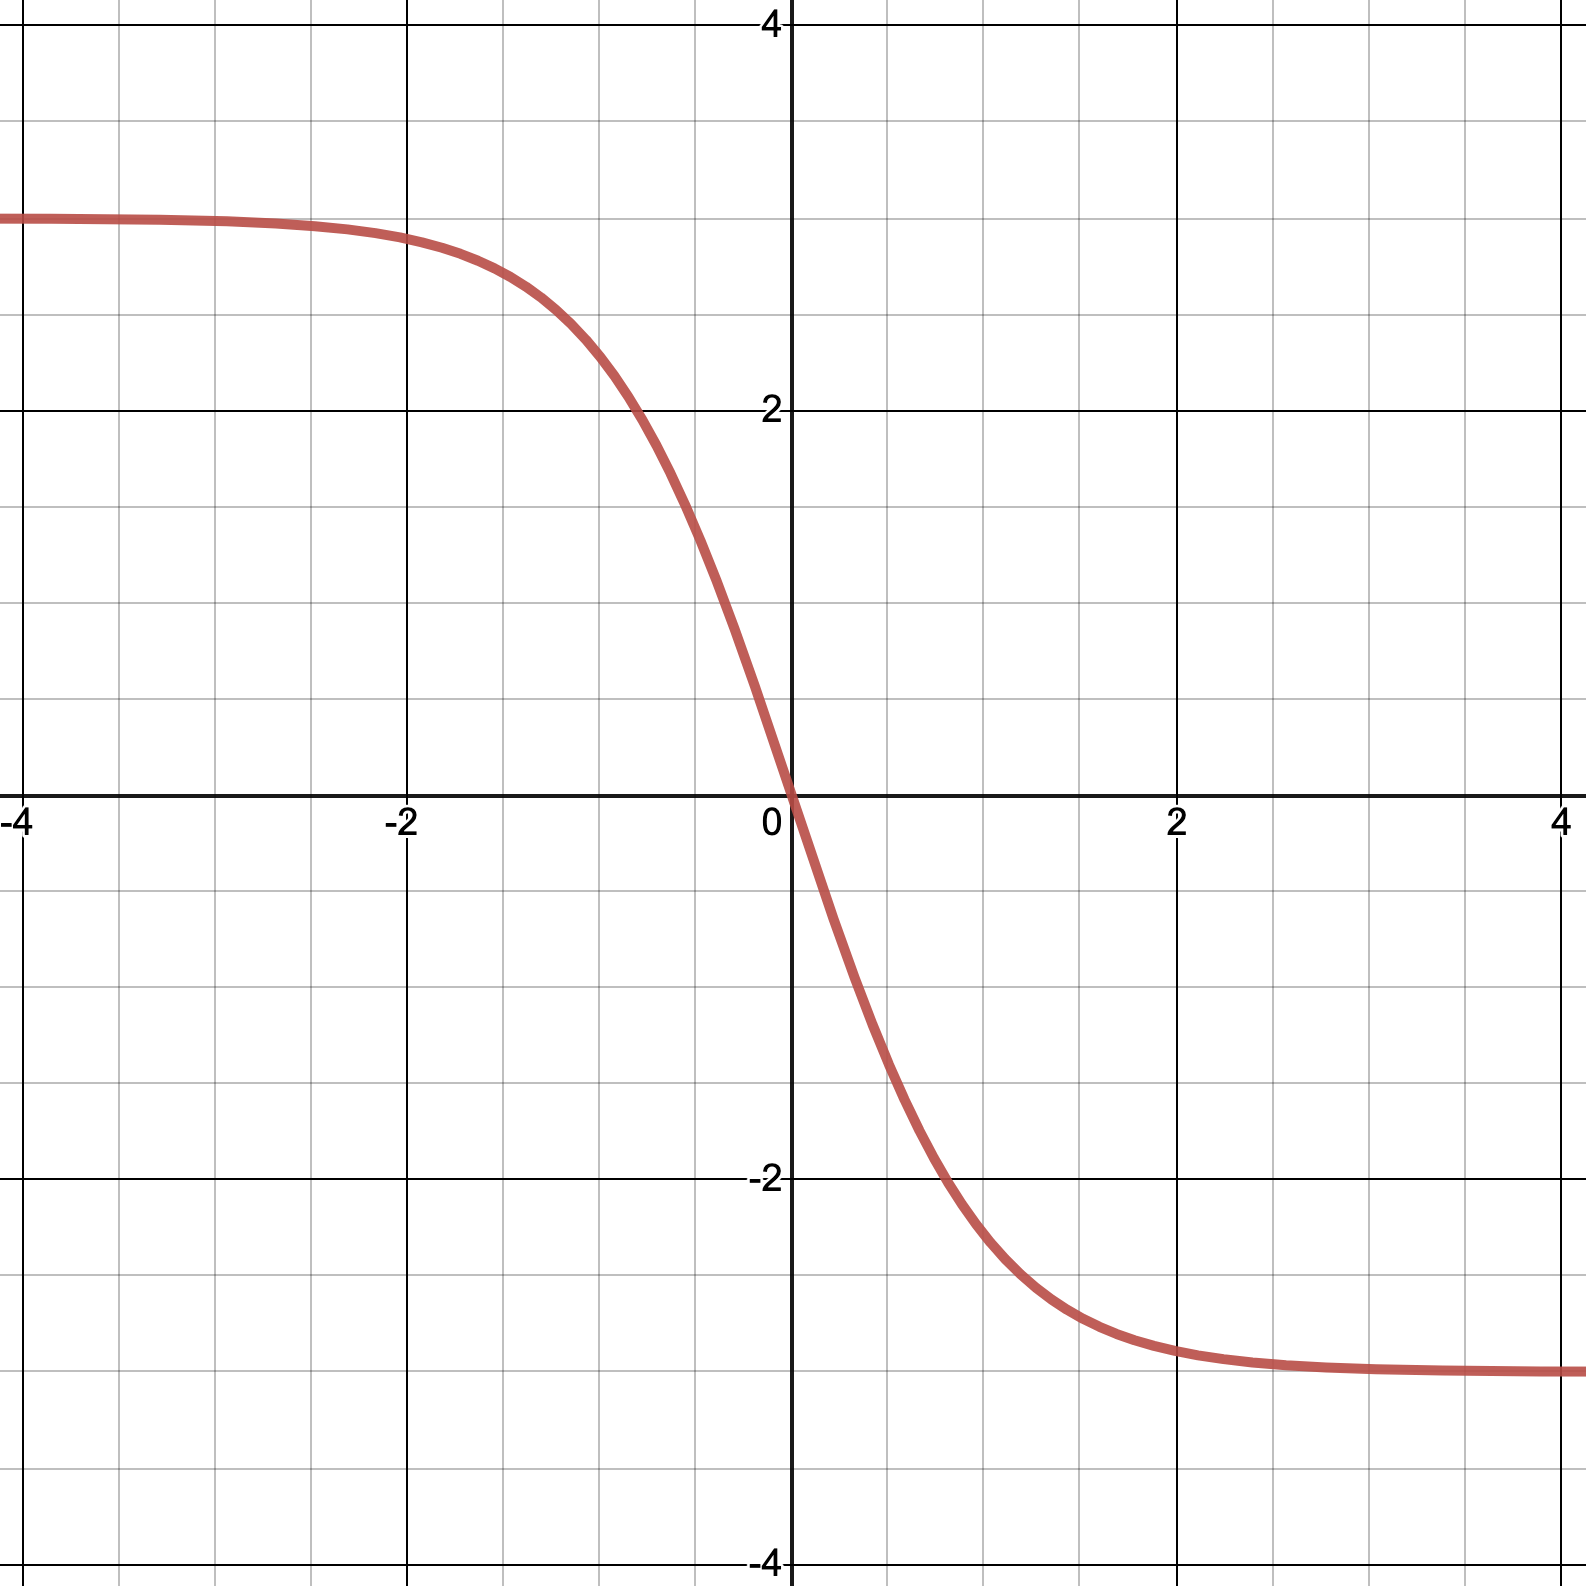
\includegraphics[width=\linewidth]{img/pt2-graph3d}
            \end{center}
            \begin{center}
                Graph I
                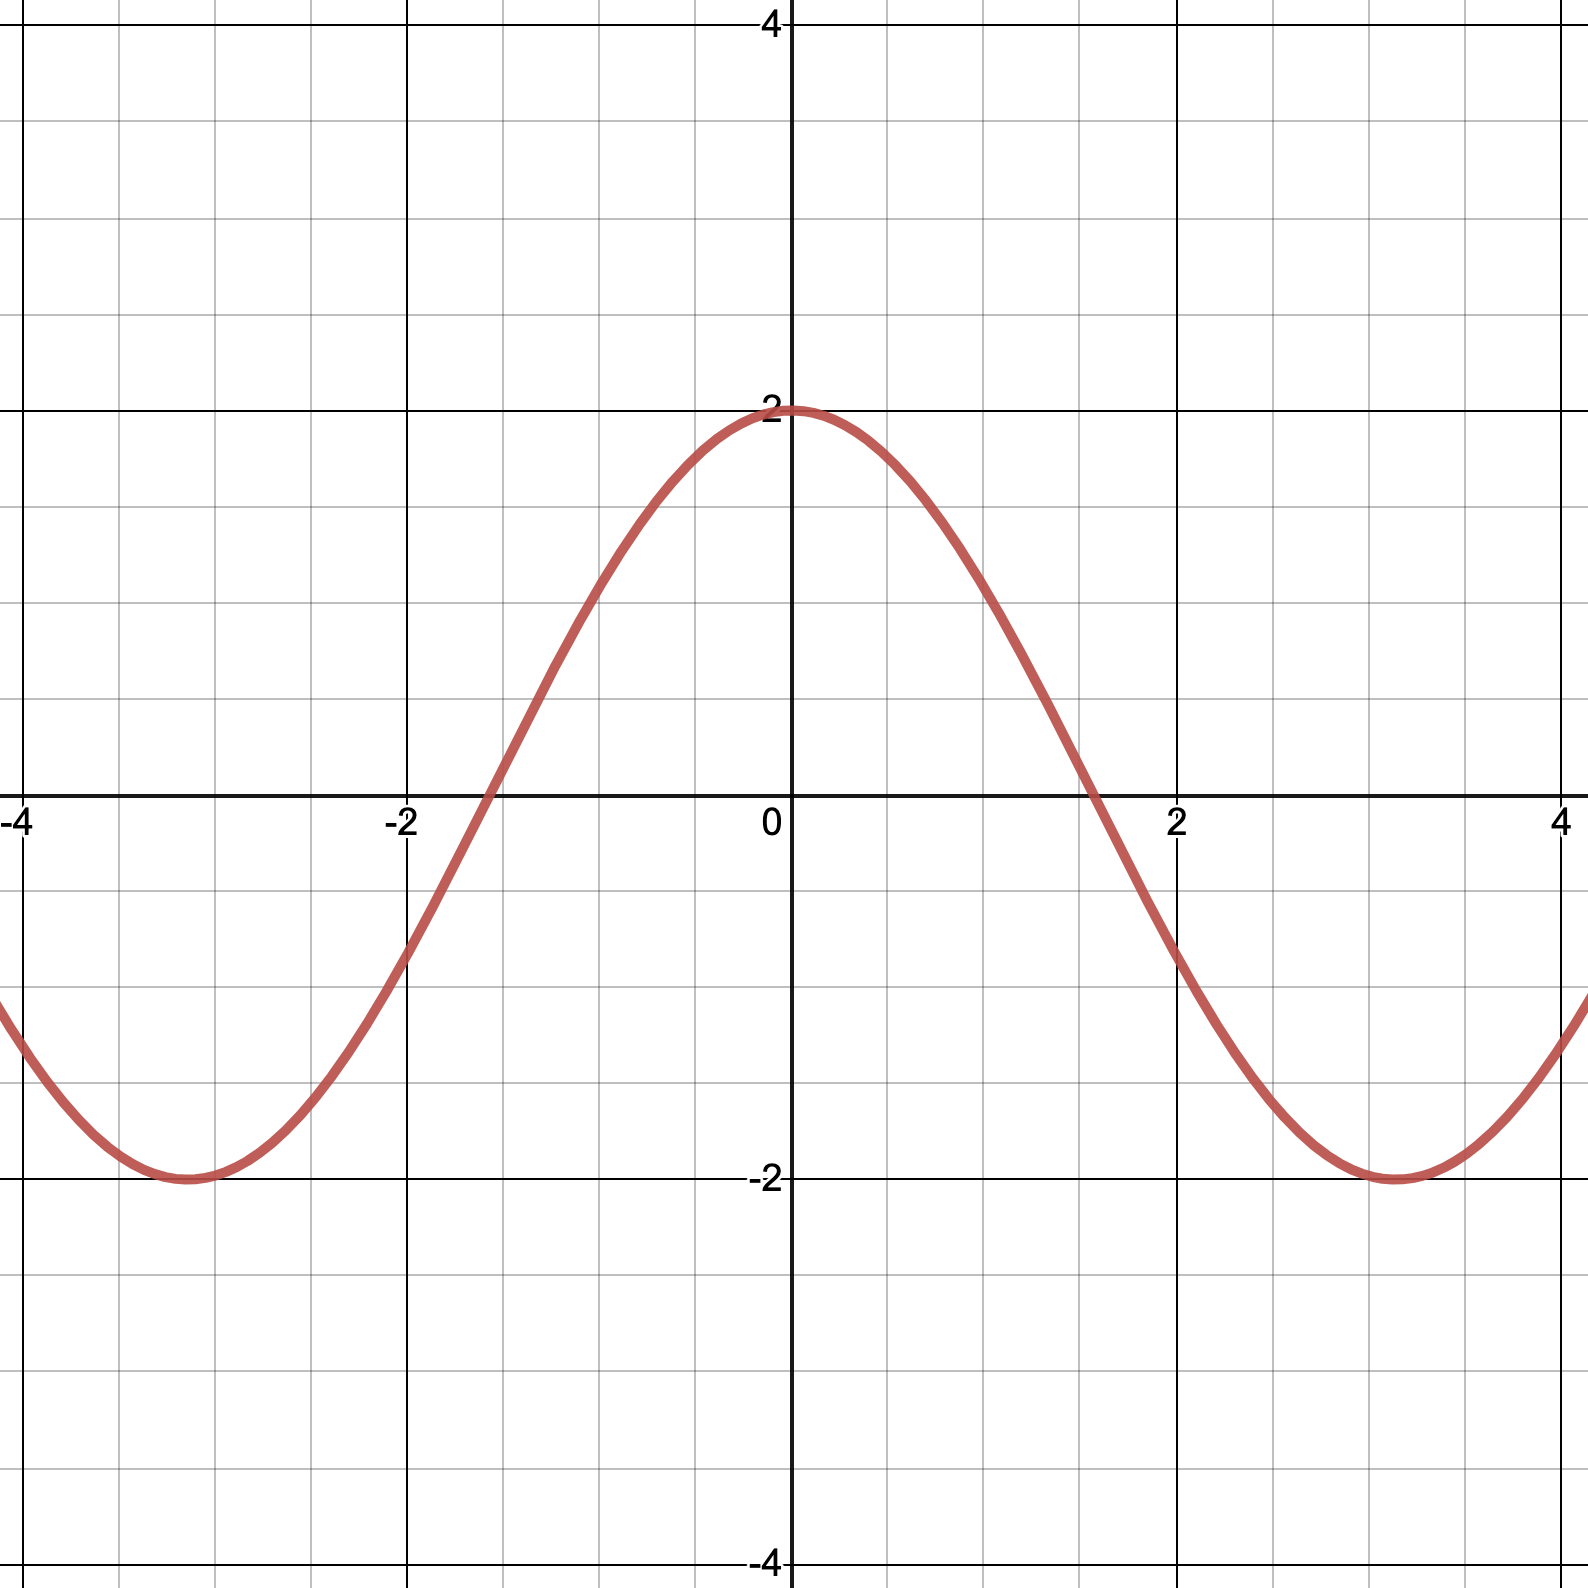
\includegraphics[width=\linewidth]{img/pt2-graph3h}
            \end{center}
        \end{multicols}
        \vspace{-1cm}
        \begin{multicols}{3}
            \begin{center}
                $$f(x)=\underline{\hspace{2cm}}$$
                $$f'(x)=\underline{\hspace{2cm}}$$
                $$f''(x)=\underline{\hspace{2cm}}$$
            \end{center}
            \begin{center}
                $$g(x)=\underline{\hspace{2cm}}$$
                $$g'(x)=\underline{\hspace{2cm}}$$
                $$g''(x)=\underline{\hspace{2cm}}$$
            \end{center}
            \begin{center}
                $$h(x)=\underline{\hspace{2cm}}$$
                $$h'(x)=\underline{\hspace{2cm}}$$
                $$h''(x)=\underline{\hspace{2cm}}$$
            \end{center}
        \end{multicols}
    \end{multipartquestion}
    \newpage
    
    \begin{multipartquestion}{Using the table below, compute the derivative of the following functions.}
        
        \begin{center}
            \begin{tabular}{|c|c|c|c|c|}
                \hline
                \textbf{$x$} & \textbf{$f(x)$} & \textbf{$f'(x)$} & \textbf{$g(x)$} & \textbf{$g'(x)$} \\ \hline
                     0       &        0        &        1         &        2        &        4         \\ \hline
                     2       &       -1        &        3         &       -1        &        2         \\ \hline
                     4       &        3        &        0         &        5        &        1         \\ \hline
            \end{tabular}
        \end{center}
    
        \frq{$a(x)=f(x)g(x)$; $~~~a'(2)$}
        \Smallsp
        \frq{$b(x)=f(\ln(2x-3))+\dfrac{g(2x)}{x}$; $~~~b'(2)$}
        \Smallsp
        \frq{$c(x)=f(g(\sin(x)))$; $~~~c'(0)$}
        \Smallsp
        \frq{$d(x)=x^2f(x)+e^xg(x)$; $~~~d'(4)$}
        \Smallsp
        
    \end{multipartquestion}
    \newpage
    
    \mcq{Compute the derivative of each of the following functions. \underline{You do not need to simplify your answers}.}{
        \task $g(x)=(3x-5e^x)^4$
        \Smallsp
        \task $f(x)=e^{x^2-3x}-\cos\left(\ln(1)\right) $
        \Smallsp
        \task $h(t)=\sqrt{-2+\dfrac{2}{3t^2}}$
        \Smallsp
        \task $Q(r)=(1-r)^{1/r}$
        \Normalsp   
        \task $f(x)=\ln(\sec(x^2))$
        \normalsp
        \task $g(t)=\arccos(t^3)$
        \Smallsp 
        \task $f(x)=\dfrac{3x^7-5}{2x}$
        \Smallsp
        \task $f(x)=e^{-x}\sqrt{1-e^x}$
        \Smallsp
        \task $g(t)=\arccot(3t^2)$
        \Smallsp
        \task $h(x)=(\csc(x))^x$
        \Normalsp
        \task $T(x)=\dfrac3x+\sqrt{-2+x^2}$
        \Normalsp
        \task $f(x)=\cos(x^2)\sin(3x)\sec(e^x)$
        \Normalsp
        \task[] {\color{white} $g(x)=\arcsec(2x^3)$}
        \Normalsp
        \task $h(t)=(1+t)^{1/t}$
        \Normalsp
        \task Let $y=\sin^{-1}(3x)+2^x+\log_2x$. Find $y'(x)$. 
        \Normalsp
        \task Let $y=\sqrt{1+e^{-x}}$. Find $\dddx[y]$.
        \Normalsp
        \task Let $y=\dfrac{\sec x}{\ln x}+x^{-1}\cos(2x)$. Find $y'(x)$.
        \Normalsp 
        \task Let $x^2-xy-3y=3$. Find $\dddx[y]$ at the point $(2,1)$.
    }
    \newpage
    
    % Higher Derivatives
    \mcq{Compute the first and second derivatives of the following functions. \textbf{You do not need to simplify.}}{
        \task $f(x)=5x^2-x^3+2x^{-3}$
        \Smallsp
        \task $H(y)=y^5e^y+\pi$
        \Normalsp
    }

    % Weird Derivative
    \frq{(You do not need to simplify) Suppose $f(1)=1/2$, $f'(1)=4$, $g(1)=1/\sqrt{3}$, $g'(1)=3$. Find $H'(1)$ where}
    $$H(x)=\frac{1-x}{f(x)}-x^3f(x^2)-\arcsin(g(x))$$
    \newpage
    
    % Implicit
    \frq{Determine $\dddx[y]$ where}
    $$\arccos(y)+\frac{8}{y}=2x^2+12e^x$$
    \Normalsp
    
    % Physics
    \begin{multipartquestion}
        A rock thrown vertically upward from the surface of the moon has a velocity of $24$m/s reaches a height of $s(t)=24t-0.8t^2$ m in $t$ seconds.
        \frq{What is the velocity of the rock at the moment it hits the surface of the moon?}
        \normalsp
        \frq{What is the acceleration due to gravity on the moon?}
        \Normalsp
    \end{multipartquestion}
    \newpage

    % Derivative with Table
    \frq{Use the information given in the chart and the function $H(x)$ below to find $H'(2)$. \textbf{Simplify your answer as much as possible.}}
    \begin{multicols}{2}
        $$H(x)=\dfrac{g(x)}{\ln(f(x))}$$\\
        \begin{tabular}{|c|c|c|c|c|}
            \hline
            $x$ & $f(x)$ & $f'(x)$ & $g(x)$ & $g'(x)$ \\
            \hline
            $2$ & $e^2$ & $\pi$ & $e^3$ & $1/2$\\
            \hline
        \end{tabular}
    \end{multicols}
    \Normalsp

    % Derivative with table and graph
    \frq{Use the information give and the function $f(x)$ below to find $f'(2)$. \textbf{Simplify your answer as much as possible.}}
    \begin{multicols}{2}
        $$a(x)=x^3-8x$$
        
        \begin{center}
            \begin{tabular}{|c|c|c|c|c|c|c|}
                \hline
                $x$ & -4 & -2 & 0 & 2 & 4 & 6\\
                \hline
                $b(x)$ & $-7$ & 0 & 2 & 0 & $-\pi$ & 3 \\
                \hline
                $b'(x)$ & $-3$ & $-2$ & 0 & $4$ & $-2$ & $2$\\
                \hline
            \end{tabular}
        \end{center}
    
        \begin{center}
            \mbox{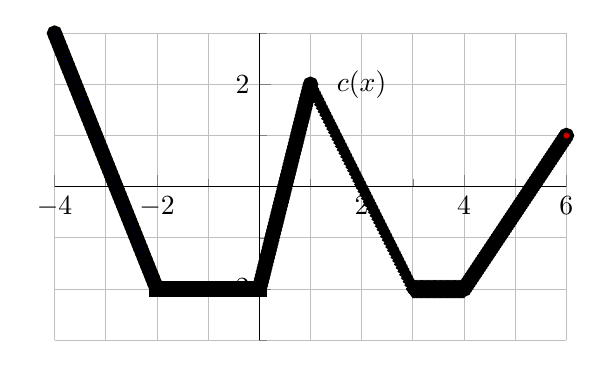
\begin{tikzpicture}[baseline=(current bounding box.north)]
                \begin{axis}[
                x=0.65cm,
                y=0.65cm,
                xmin=-4,
                xmax=6,
                ymin=-3,
                ymax=3,
                grid=both,
                major grid style={line width=.2pt,draw=gray!50},
                minor tick num=1,
                axis x line*=middle,
                axis y line*=middle,
                every axis plot/.append style={ultra thick},
                samples=60
                ]
                \addplot+[black, domain=-4:-2] {-2.5*x-7};
                \addplot+[black, domain=-2:-0] {-2};
                \addplot+[black, domain=0:1] {4*x-2};
                \addplot+[black, domain=1:3] {-2*x+4};
                \addplot+[black, domain=3:4] {-2};
                \addplot+[black, solid, domain=4:6] {3/2*x-8};
                \node at (2,2) {$c(x)$};
                \end{axis}
                \end{tikzpicture}}
        \end{center}
    \end{multicols}
    $$f(x)=\ln(a(x))+b(-2x)c(x)$$
    \newpage

    % Implicit differentiation and application
    \mcq{Consider the curve given by the following equation. $$x+\frac{17}{x}=2y^2+12y$$}{
        \task Determine $\dddx[y]$.
        \Largesp
        \task Find all values of $x$ at which the curve has a vertical tangent line.
        \Largesp
    }
\newpage

    % Derivatives from graphs
    \begin{multipartquestion}
        Consider the graph of $f$ shown below.
        \begin{center}
        \mbox{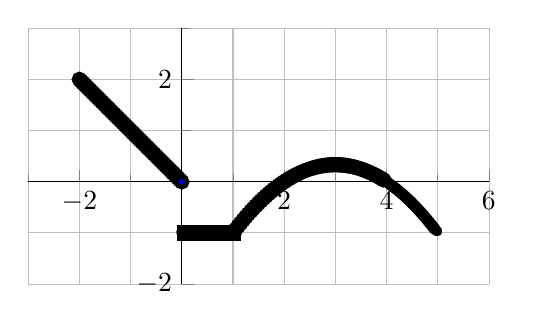
\begin{tikzpicture}[baseline=(current bounding box.north)]
            \begin{axis}[
            x=0.65cm,
            y=0.65cm,
            xmin=-3,
            xmax=6,
            ymin=-2,
            ymax=3,
            grid=both,
            major grid style={line width=.2pt,draw=gray!50},
            minor tick num=1,
            axis x line*=middle,
            axis y line*=middle,
            every axis plot/.append style={ultra thick},
            samples=60
            ]
            \addplot+[black, domain=-2:0] {-x};
            \addplot+[black, domain=0.06:1] {-1};
            \addplot+[black, domain=1:3.94] {-1/3*(x-3)^2+1/3};
            \addplot+[black, domain=4.06:4.94] {-1/3*(x-3)^2+1/3};
            \node at (-2,2) {$\circ$};
            \node at (0,-1) {$\circ$};
            \node at (4,0) {$\circ$};
            \node at (0,0) {\textbullet};
            \node at (5,-1) {\textbullet};
            \end{axis}
            \end{tikzpicture}}
        \end{center}
        \frq{Find all values of $x$ in $[-2, 5]$ such that $f'(x)=0$.}
        \Tinysp
        \frq{Find all values of $x$ in $[-2, 5]$ such that $f'(x)$ is undefined.}
        \Tinysp
        \frq{Find $\lim\limits_{h\to 0}\dfrac{f(h-1)-f(-1)}{h}$.}
        \Tinysp
    \end{multipartquestion}
    
    \frq{Find the derivative of $g(x)=x^{\sin x}$.}
    \newpage
    
    % Related Rates
    \frq{Evil McScquiivel just robbed the ReallyRich Bank and is driving north in his getaway car at a speed of 60 mph. The cops are following him northbound when Mr. McScquiivel turns east. When the cops are 3 mi from the intersection and Mr. McScquiivel is 4 mi from the intersection, the rate of change of the distance between the cars is $-28$ mph. What is the speed of the cop car?}
    \hugesp
    \frq{Your cat Jimmy was playing on your kitchen counter when he accidentally knocked over a salt shaker. Bad Jimmy. The salt shaker pours salt over the counter at a rate of $\SI{3}{\centi\meter^3/\second}$, which collects into a cone of salt on the ground. At any point in time, the height of the cone is always equal to its diameter. What is the rate of change of the radius of the cone of salt at the moment when its height is $\SI{2}{\centi\meter}$?}
    \newpage
\end{document}